\documentclass[14pt, a4paper]{article}
\usepackage[utf8]{inputenc}
\usepackage[russian]{babel}
\usepackage{graphicx}

\title{\textbf{Отчет о выполнении лабораторной работы 1.2.2}}
\author{Калашников Михаил, Б03-205}
\date{}

\begin{document}

\maketitle

В работе использовались крестообразный маятник, набор перегрузов, линейка, компьютер с лазерной установкой для измерения положения маятника.

\begin{enumerate}

\item С помощью перемещения грузов вдоль стержней маятника, добьемся положения безразличного равновесия. При этом среднее расстояние грузов от оси $R=10.75\ cm$.

\item Запишем основные параметры установки в таблицу \ref{table1}.

\begin{table}[!h]
\centering
\begin{tabular}{| c | c |}
\hline
Масса платформы $m_0$ & $24.915\ g$ \\
Средняя масса грузов $m_1$ & $151.6\ g$ \\
Радиус грузов $R_1$ & $16\pm1\ mm$ \\
Высота грузов $l$ & $25\pm1\ mm$ \\
Высота опускания грузов $h$ & $93\pm0.1\ cm$ \\
Радиус малого шкива $r_1$ & $0.90\pm0.01\ cm$ \\
Радиус большого шкива $r_2$ & $1.85\pm0.01\ cm$ \\
\hline
\end{tabular}
\caption{Основные параметры установки}
\label{table1}
\end{table}


\item Измерения занесем в таблицу \ref{table2}. Рассчитаем среднее время $\bar{t}$, угловое ускорение $\beta$, момент силы натяжения $M_T$:

\[\bar{t}=\frac{\sum_{k=1}^{N}t_k}{N},\ \beta=\frac{2h}{rt^2},\ M_T=mr(g-r\beta).\]

Погрешность измерений времени может быть найдена как среднеквадратическое отклонение:

\[\sigma_t=\sqrt{\frac{\sum_{k=1}^N(t-\bar{t})^2}{N(N-1)}}.\]

Погрешности остальных измерений могут быть найдены по общей формуле:

\[\sigma_Y=\sqrt{\sum_{i=1}^N\left(\frac{\delta Y}{\delta X_i}\sigma_{X_i}\right)^2}.\]

Таким образом,

\[\sigma_{\beta}=\sqrt{\left(\frac{2}{rt^2}\sigma_h\right)^2+\left(\frac{2h}{r^2t^2}\sigma_r\right)^2+\left(\frac{4h}{rt^3}\sigma_t\right)^2}=\beta\sqrt{\left(\frac{\sigma_h}{h}\right)^2+\left(\frac{\sigma_r}{r}\right)^2+\left(2\frac{\sigma_t}{t}\right)^2};\]

\[\sigma_{M_T}=\sqrt{\left(m(g-2r\beta)\sigma_r\right)^2+\left(mr^2\sigma_{\beta}\right)^2}.\]

\begin{table}[!h]
\centering
\begin{tabular}{| c | c | c | c | c | c | c | c |}
\hline
Диаметр & Масса & \multicolumn{3}{| c |}{} & & & \\
шкива, $cm$ & перегрузка, $g$ & \multicolumn{3}{| c |}{Время падения, $s$} & $\bar{t}\pm\sigma_{\bar{t}},\ s$ & $\beta\pm\sigma_{\beta},\ s^{-2}$ & $M_T\pm\sigma_{M},\ g\cdot m^2$ \\
\hline
0.90 & 69.52 & 21.90 & 22.37 & 22.25 & $22.17\pm 0.141$ & $0.42\pm 0.007$ & $6.14\pm 0.068$ \\
\hline
0.90 & 83.56 & 19.94 & 19.92 & 19.61 & $19.82\pm 0.107$ & $0.53\pm 0.008$ & $7.38\pm 0.082$ \\
\hline
0.90 & 98.54 & 17.00 & 17.15 & 16.90 & $17.02\pm 0.073$ & $0.71\pm 0.010$ & $8.70\pm 0.097$ \\
\hline
0.90 & 124.91 & 14.60 & 14.67 & 15.30 & $14.86\pm 0.223$ & $0.94\pm 0.030$ & $11.03\pm 0.122$ \\
\hline
1.75 & 69.52 & 10.67 & 10.70 & 10.49 & $10.62\pm 0.066$ & $0.94\pm 0.013$ & $11.92\pm 0.068$ \\
\hline
1.75 & 83.56 & 9.61 & 9.40 & 9.65 & $9.55\pm 0.078$ & $1.16\pm 0.020$ & $14.32\pm 0.082$ \\
\hline
1.75 & 98.54 & 8.22 & 8.57 & 8.46 & $8.42\pm 0.103$ & $1.50\pm 0.038$ & $16.88\pm 0.096$ \\
\hline
1.75 & 124.91 & 7.48 & 7.23 & 7.16 & $7.29\pm 0.097$ & $2.00\pm 0.055$ & $21.38\pm 0.122$ \\
\hline

\end{tabular}
\caption{Результаты измерения времени падения груза}
\label{table2}
\end{table}

\item Построим график зависимости $M_T(\beta)$ (рис. \ref{image1}). Зная, что $M_T=M_{fr}+\beta I$, найдем с помощью метода наименьших квадратов параметры $M_{fr}$ и $I$. Для $r=1.75\ cm$ получим значения:

\[M_{fr}=3.81\ mN\cdot m,\ I=8.78\ g\cdot m^2.\]

\item Занесем результаты экспериментов с различными моментами инерции в таблицу \ref{table3}. Повторим для них вычисления, описанные в предыдущих пунктах, используя полученную величину $M_{fr}$. Значения $\bar{t}$, $\beta$, $M_T$, $I$ запишем в таблицу \ref{table4}. 

\[I=\frac{M_T-M_{fr}}{\beta}\]

\[\sigma_I=I\sqrt{\left(\frac{\sigma_{M_T}}{M_T-M_{fr}}\right)^2+\left(\frac{\sigma_{\beta}}{\beta}\right)^2}\]

На основе полученного значения $I_0=I(R=0)=4.20\pm 2.43\ g\cdot m^2$, рассчитаем $I_{th}$ по формуле:

\[I_{th}=I_0+4m_1R^2+\frac{1}{3}m_1l^2+m_1R_1^2.\]

\[\sigma_{I_{th}}=\sqrt{\sigma_{I_0}^2+\left(8m_1R\sigma_R\right)^2+\left(\frac{2}{3}m_1l\sigma_l\right)^2+\left(2m_1R_1\sigma_{R_1}\right)^2}\]

\begin{table}[!h]
\centering
\begin{tabular}{| c | c | c | c | c | c | c |}
\hline
Радиус & Масса & Расстояние до & & & & \\
шкива, $r,\ cm$ & перегрузка, $m,\ g$ & грузов, $R,\ cm$ & $t1,\ s$ & $t2,\ s$ & $t3,\ s$ & $t4,\ s$ \\
\hline
1.75 & 62.9 & 20.5 & 14.69 & 14.50 & 14.55 & 15.00 \\
\hline
1.75 & 62.9 & 17.2 & 13.00 & 12.70 & 12.81 & 13.38 \\
\hline
1.75 & 62.9 & 6.6 & 8.50 & 8.30 & 8.49 & 8.34 \\
\hline
1.75 & 62.9 & 3.5 & 7.01 & 6.97 & 7.35 & 7.42 \\
\hline
1.75 & 62.9 & 0.0 & 6.37 & 6.24 & 6.19 & 6.45 \\
\hline
\end{tabular}
\caption{Результаты экспериментов с различными моментами инерции системы}
\label{table3}
\end{table}

\begin{table}[!h]
\centering
\begin{tabular}{| c | c | c | c | c | c |}
\hline
Расстояние до & & & & & \\
грузов, $R,\ cm$ & $\bar{t},\ s$ & $\beta, s^{-2}$ & $M_T,\ mN\cdot m$ & $I,\ g\cdot m^2$ & $I_{th},\ g\cdot m^2$ \\
\hline
20.50 & $14.68\pm 0.11$ & $0.49\pm 0.01$ & $15.07\pm 0.09$ & $22.84\pm 0.41$ & $29.75\pm 0.49$ \\
\hline
17.20 & $12.97\pm 0.15$ & $0.63\pm 0.01$ & $15.07\pm 0.09$ & $17.82\pm 0.44$ & $22.21\pm 0.50$ \\
\hline
6.60 & $8.41\pm 0.05$ & $1.50\pm 0.02$ & $15.04\pm 0.09$ & $7.47\pm 0.12$ & $6.91\pm 0.16$ \\
\hline
3.50 & $7.19\pm 0.12$ & $2.06\pm 0.07$ & $15.03\pm 0.09$ & $5.45\pm 0.18$ & $5.01\pm 0.20$ \\
\hline
0.00 & $6.31\pm 0.06$ & $2.67\pm 0.05$ & $15.01\pm 0.09$ & $4.20\pm 0.09$ & - \\
\hline
\end{tabular}
\caption{Обработанные результаты экспериментов с различными моментами инерции системы}
\label{table4}
\end{table}

\item Построим график зависимости $I(R^2)$ (рис. \ref{image2}).
Значение $I(0)$ соответствует ситуации, когда грузы расположены на оси вращения маятника и не вносят вклад в момент инерции системы. То есть:
\[I(0)=5.29\ g\cdot m^2.\]

Это значение учитывает в себе поправку $\Delta I=\frac{1}{3}m_1l^2+m_1R_1^2=0.07\ g\cdot m^2$. Если ее вычесть, то получим, что

\[I_{0lin}=I(0)-\Delta I=5.22\ g\cdot m^2.\]

\end{enumerate}

\begin{figure}
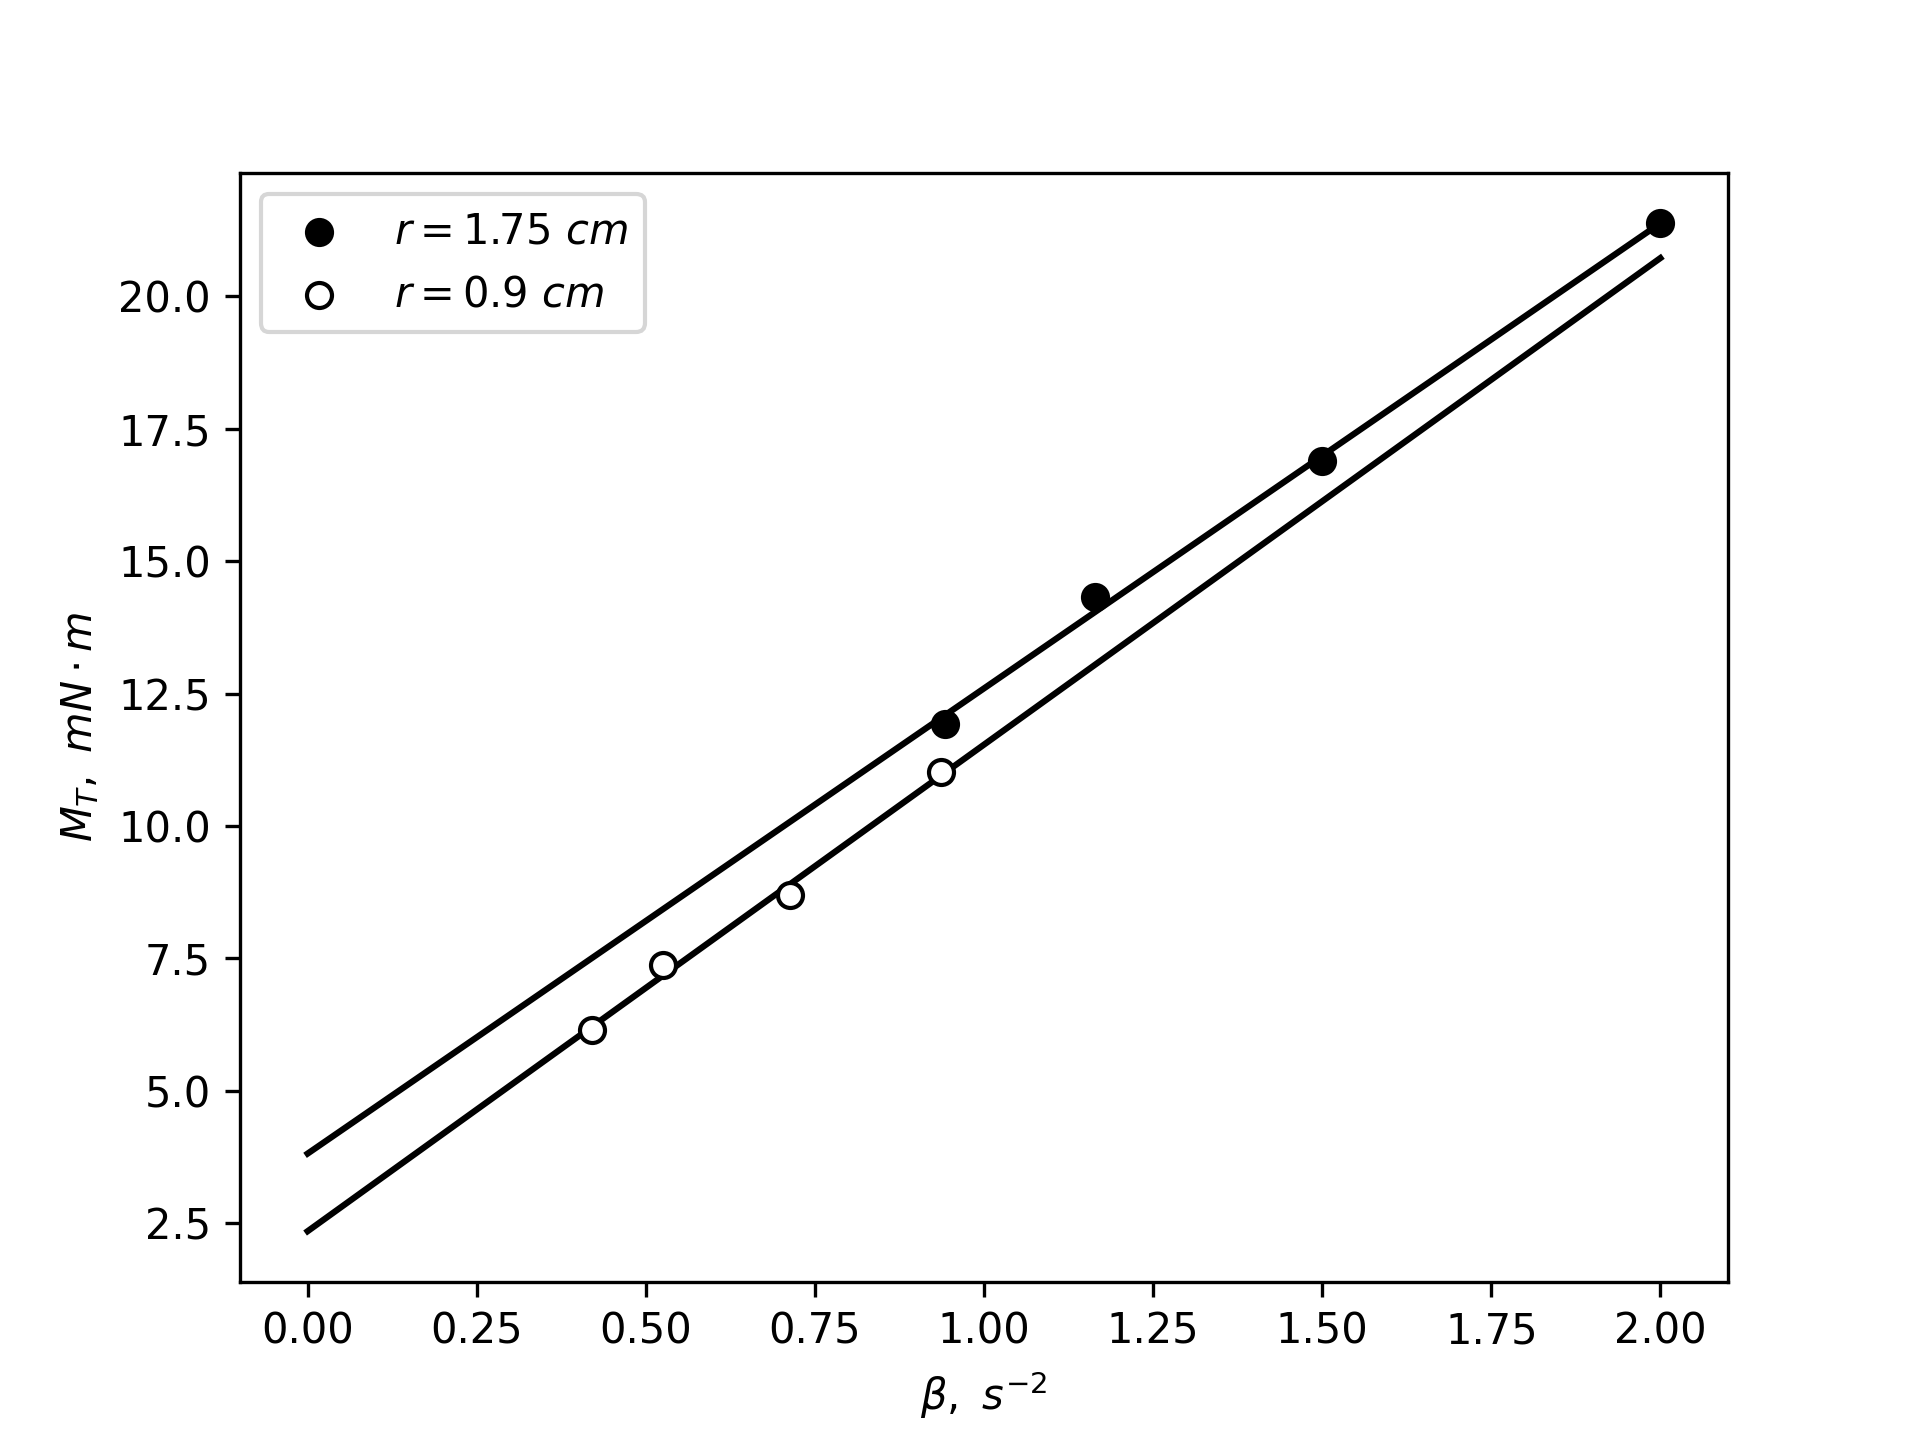
\includegraphics[width=\linewidth]{laba3_1.png}
\caption{График зависимости $M_T(\beta)$}
\label{image1}
\end{figure}

\begin{figure}
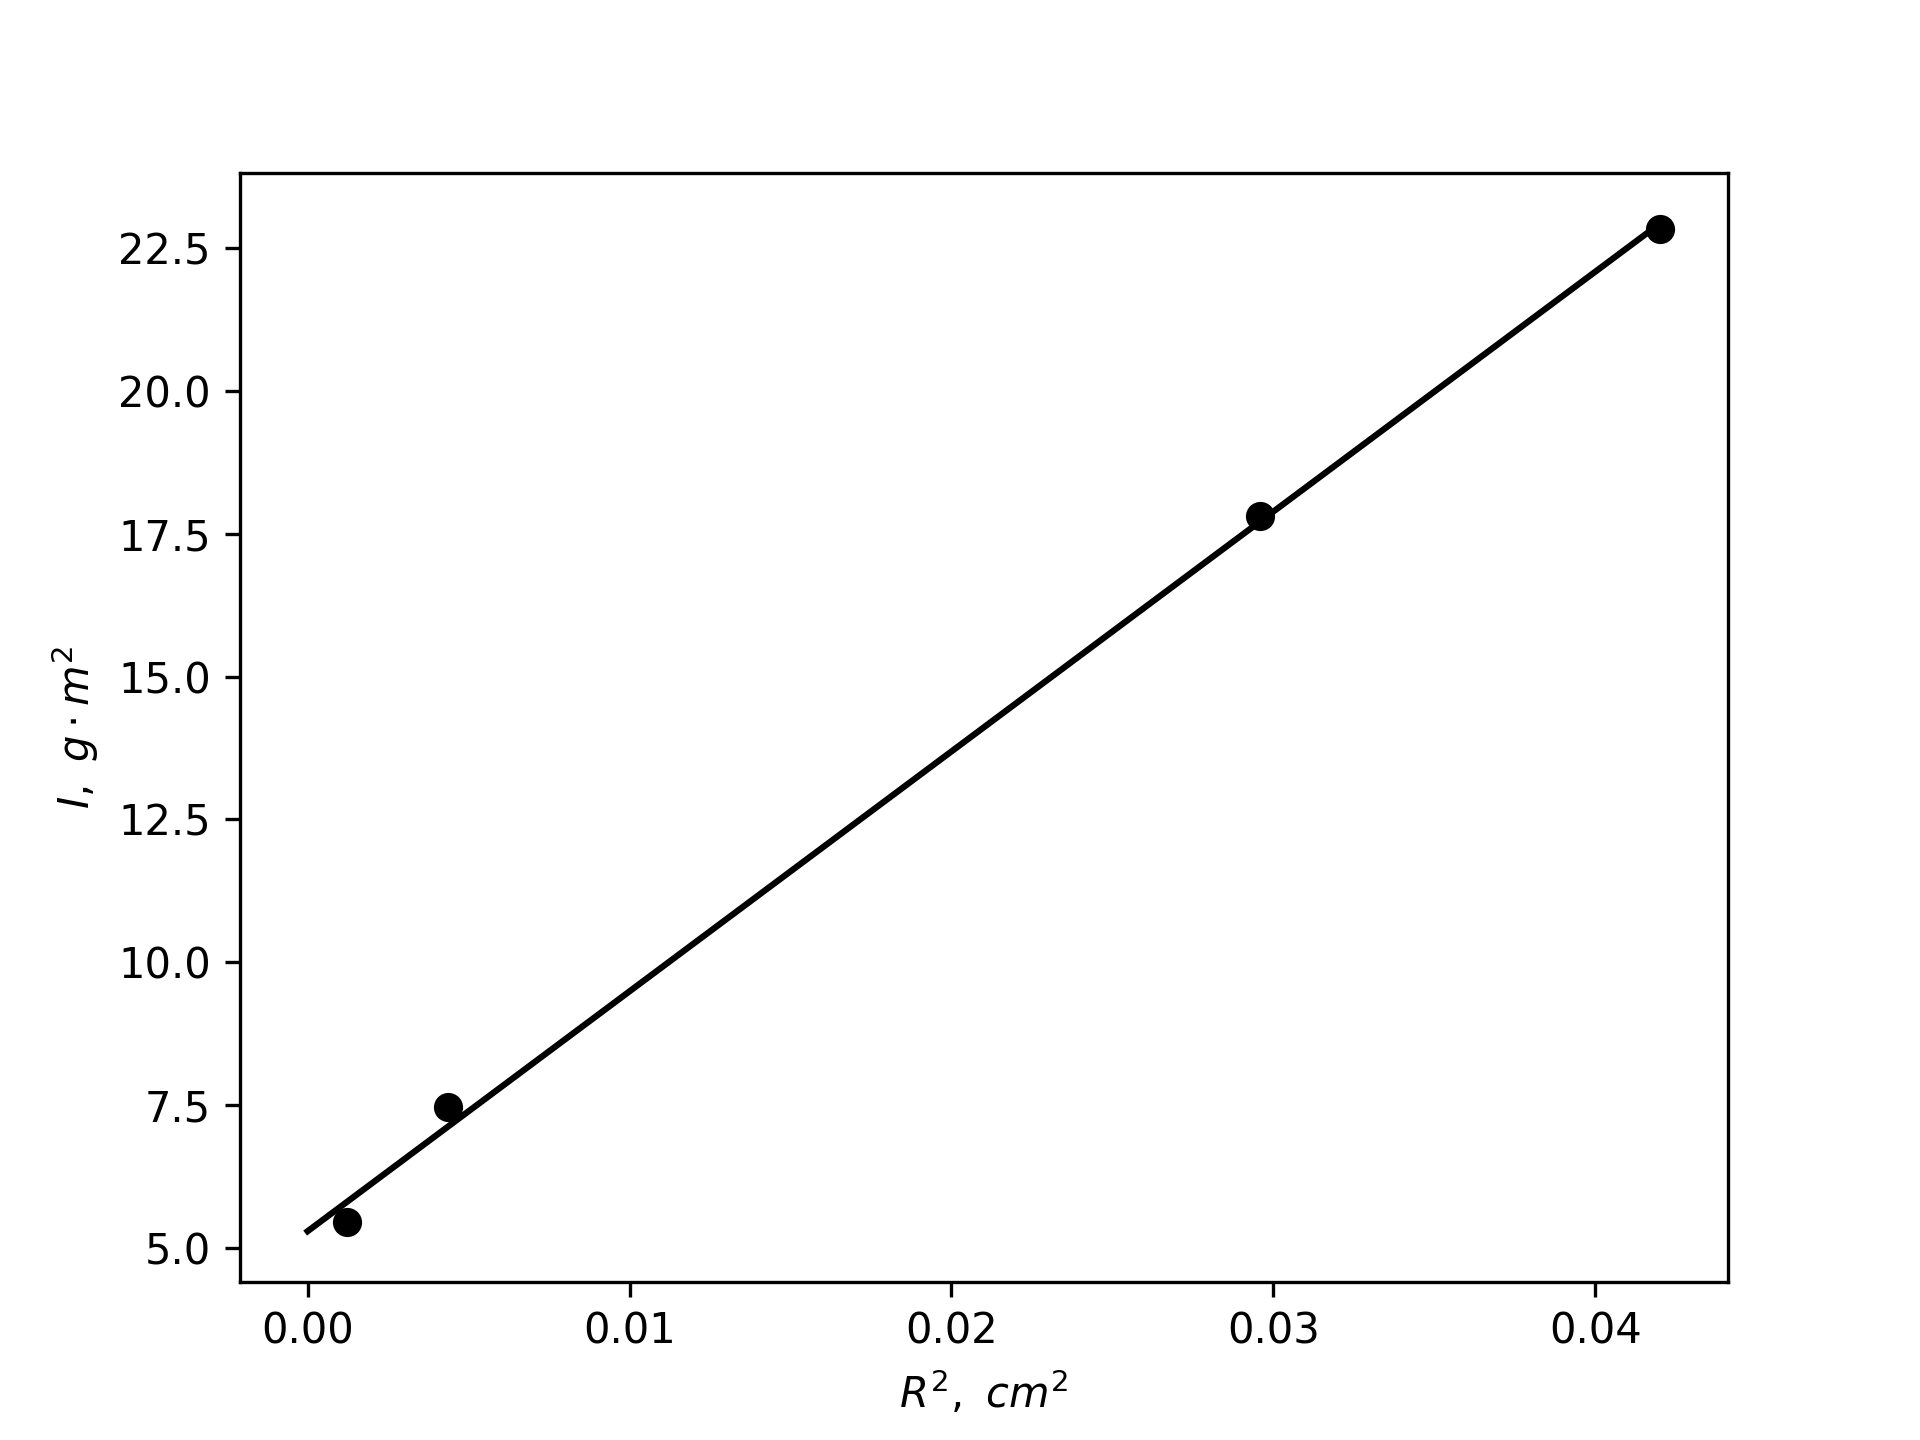
\includegraphics[width=\linewidth]{laba3_2.png}
\caption{График зависимости $I(R^2)$}
\label{image2}
\end{figure}

\end{document}